% !TeX root = ../main.tex
% -*- coding: utf-8 -*-

\chapter{基于近边界数据的模型所有权推断方法分析}\label{5}

本文在三个开源数据集上进行实验,选择ResNet18作为评估的源模型,VGG11作为对照的无关模型。本章将从初始近边界数据的生成算法、近边界数据私有化方法、近边界数据的可继承性、源模型微调的影响、模型所有权推断的有效性和近边界数据规模的可伸缩性这几个方面对本文提出的方法进行评估和分析。本文采用了几种主流的模型窃取攻击方法,包括模型微调,模型剪枝(不同的剪枝率)和模型知识蒸馏,并在源模型的基础上派生得到盗窃模型。

\section{实验设置}\label{5.1}

\subsection{数据集}

\noindent\textbf{CIFAR-10\cite{krizhevsky2009learning}:}CIFAR-10共有10个类别,其中训练集包含50000张大小为32x32的图像,测试集包含10000张大小为32x32的图像。

\noindent\textbf{Heritage\footnote{https://datahub.io/dataset/architectural-heritage-elements-image-dataset}:}Heritage共有10个类别,其中训练集包含10235张大小为128x128的图像,测试集包含1404张大小为64x64的图像。

\noindent\textbf{Intel\_image\footnote{https://www.kaggle.com/datasets/puneet6060/intel-image-classification}:}Intel\_image共有6个类别,其中训练集包含14034张大小为150x150的图像,测试集包含3001张大小为150x150的图像。

\subsection{实验环境和参数设置}

\textbf{(1)实验环境}

本文在实验中使用的硬件与软件配置如表\ref{table:11}所示,实验使用的机器配备16核Intel i7-11700KF CPU、NVIDIA GeForce RTX 3080 Ti显卡、16GB 内存以及Ubuntu 20.04 LTS操作系统,实验代码均使用Python语言和Pycharm工具基于Pytorch框架实现。

\begin{table}[H]
	\centering
%	\setlength{\arrayrulewidth}{0.5mm}
	\renewcommand\arraystretch{1.2}
	\caption{硬件与软件配置}
	\label{table:11}
	\small
	\begin{tabular*}{13cm}{@{\extracolsep{\fill}} l c }
%		\hline
		\toprule[1pt]
		\textbf{硬件/软件}      &   \textbf{配置}    \\
		\hline
%		\toprule[0.5pt]
		操作系统  &   Ubuntu 20.04 LTS    \\
		
		CPU     &   Intel Core i7-11700KF @ 3.6GHz       \\
		
		内存     &   16GB       \\
		
		显卡     &   NVIDIA GeForce RTX 3080 Ti \\
		
		CUDA版本     &   	11.6          \\
		
		深度学习框架     &   Pytorch 1.9.0          \\
		
		开发工具    &   Pycharm         \\
		
		开发语言     &   Python 3.7.11           \\
		
		\bottomrule[1pt]
%		\hline		
	\end{tabular*}
\end{table}

\textbf{(2)参数设置}

\textbf{源模型训练:}训练过程中使用Adam优化器并将学习率(Learning rate),训练轮次(Epoch)和每批次大小(Batch size)分别设置为0.0001,200和64,其他参数为默认值。

\textbf{模型蒸馏:}蒸馏模型实验选择从Resnet18蒸馏至VGG11,蒸馏时将蒸馏温度设置为20并且教师模型比例$\alpha$=0.7,训练过程中使用Adam优化器并将学习率,训练轮次和每批次大小分别设置为0.0001,20和64,其他参数为默认值。

\textbf{模型微调:}蒸馏模型实验选择固定模型其他层参数,重置全连接层参数进行微调,训练过程中使用Adam优化器并将学习率,训练轮次和每批次大小分别设置为0.0001,10和64,其他参数为默认值。

\textbf{模型剪枝:}分别以10\%,30\%,50\%的剪枝率对源模型权重进行剪枝,其他参数为默认值。

\textbf{初始近边界数据生成算法:}初始近边界数据生成采用改进的$CW$-$L_2$算法,选择有目标的生成方式,指定生成样本类别。训练过程中使用Adam优化器并将学习率,训练轮次和每批次大小分别设置为0.001,1000和64,,二分搜索次数设置为6,其他参数为默认值。

\textbf{近边界数据私有化方法:}私有近边界数据生成器采用DCGAN的基础结构,训练过程中使用Adam优化器并将学习率,训练轮次和每批次大小分别设置为0.0002,2000和64,其他参数为默认值。

本方法最后微调源模型阶段需要交替使用源模型损失函数和新设计的损失函数微调源模型,具体设置为10个轮次交替一次且交替次数最多为10次。

\subsection{源模型和盗窃模型}

本节模型训练过程中参数设置与上一小节保持一致。

\textbf{(1)源模型和无关模型}

本文的目标模型选用ResNet18网络架构,在上述三个数据集上分别进行训练,作为实验源模型,使用VGG11作为无关的对照模型。ResNet18和VGG11的参数信息如表\ref{table:10}所示。

\begin{table}[H]
	\centering
	%	\setlength{\arrayrulewidth}{0.5mm}
	\renewcommand\arraystretch{1.2}
	\caption{模型参数信息}
	\label{table:10}
	%	\zihaowu
	\small
	\begin{tabular*}{13cm}{@{\extracolsep{\fill}} l c c c }
%		\hline
		\toprule[1pt]
		\textbf{模型 }     &   \textbf{层数}    &   \textbf{计算量/亿}     &   \textbf{ 参数量/百万}     \\
		\hline
		
		ResNet18  &   18     &    9.559     &    11.670     \\
		
		VGG11     &   11     &    47.022    &    132.863     \\
		
		\bottomrule[1pt]
%		\hline		
	\end{tabular*}
\end{table}

本文在数据处理阶段将统一图片尺寸更改为64,为了更好的提取到图片中的特征,提高模型准确率,所以训练的时候将原始ResNet18中首层使用的7x7卷积核改成3x3,步长和填充随之改为1,并且舍弃最大池化层。

如表\ref{table:12}所示,更改结构后ResNet18在三个数据集上的准确率得到提升。其中,模型在CIFAR-10的准确率相较于其他两个数据集提升较大,因为CIFAR-10数据集本身的尺寸为32x32,是小尺寸图片。

\begin{table}[H]
	\centering
	%	\setlength{\arrayrulewidth}{0.5mm}
	\renewcommand\arraystretch{1.2}
	\caption{模型更改结构前后准确率对比}
	\label{table:12}
	%	\zihaowu
	\small
	\begin{tabular*}{13cm}{@{\extracolsep{\fill}} l c c c }
%		\hline
		\toprule[1pt]
		\textbf{数据集 }     &   \textbf{CIFAR-10}    &   \textbf{Heritage}     &   \textbf{Intel\_image}     \\
		\hline
		
		更改前准确率  &  0.853     &    0.862     &    0.848     \\
		
		更改后准确率 &   0.886     &    0.879    &    0.854     \\
		
		\bottomrule[1pt]
%		\hline		
	\end{tabular*}
\end{table}

更改结构后,ResNet18在三个数据集上的准确率与训练轮次的关系如图\ref{模型在三个数据集上的准确率}所示,基本在训练125次之后模型收敛,准确率基本维持不变。

\begin{figure}[htb]%%图,[htbp]是浮动格式
	\centering
	%	\setlength{\abovecaptionskip}{2mm} %图片标题与图片距离
	%	\vspace{-2mm}
	%	\setlength{\belowcaptionskip}{-3mm} %调整图片标题与下文距离
	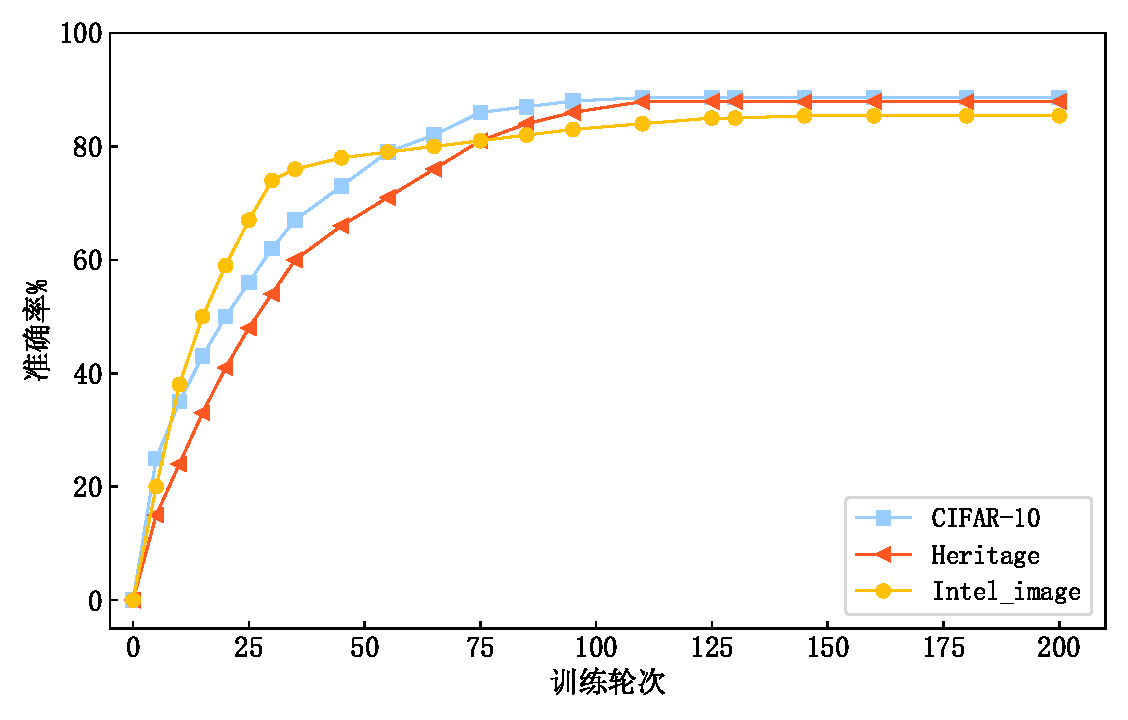
\includegraphics[width=0.9\linewidth]{准确率.pdf}
	\caption{源模型在三个数据集上的准确率}
	\label{模型在三个数据集上的准确率}
	%	\vspace{-3mm}  %调整图片标题与下文距离,与\setlength{\belowcaptionskip}{-3mm}等效。
	\end {figure}

\textbf{(2)盗窃模型}

\textbf{微调模型}:选择固定除全连接层外其余所有层的参数,将全连接层参数初始化后,进行微调作为盗窃模型。

\textbf{剪枝模型}:根据权重的$L_1$范数排序,对卷积层和全连接层分别以10\%,30\%,50\%的裁剪率进行裁剪作为盗窃模型。

\textbf{蒸馏知识}:选择蒸馏至VGG11作为盗窃模型,蒸馏时将蒸馏温度设置为20并且教师模型比例$\alpha$=0.7。
	
\section{初始近边界数据生成算法对比}\label{5.2}

本小节将对\ref{3}\ref{3.3}中提到的FGSM,IGSM,RFGSM和CW-$L_2$几种算法进行测试,评估指标为生成的初始近边界数据到分类边界的距离,距离愈小愈优。除对CW-$L_2$引入距离参数进行改进外,其余均使用原作者发布的实现。FGSM,IGSM,RFGSM中均有一个用于界定噪声$\epsilon$的参数,本文进行大量的实验探索选择合适的参数用于与CW-$L_2$进行比较。此外,CW-$L_2$的实验设置与第一节保持一致。

\begin{table}[H]
	\centering
%	\setlength{\arrayrulewidth}{0.5mm}
	\renewcommand\arraystretch{1.2}
	\caption{不同算法生成样本到分类边界的平均距离}
	\label{table:1}
	\small
	\begin{tabular*}{13cm}{@{\extracolsep{\fill}} l c c c c c}
		
%		\hline
		\toprule[1pt]
		\textbf{数据集}                 & \textbf{分组}  &   \textbf{FGSM}   &   \textbf{IGSM}   &  \textbf{RFGSM}  &   \pmb{CW-$L_2$}    \\
		\hline
\multirow{3}{6em}{CIFAR-10}    &1  &    0.557  &   0.430  &  0.418   &    \textbf{0.066}     \\
		                      & 2  &    0.461  &   0.419  &  0.373   &   \textbf{0.103}     \\
		                      & 3  &    0.586  &   0.369  &  0.356   &    \textbf{0.112 }    \\
		\hline
\multirow{3}{6em}{Heritage}   &  1 &    0.347  &   0.356  &  0.314   &    \textbf{0.014}     \\
		                      & 2  &    0.377  &   0.340  &  0.281   &    \textbf{0.016}     \\
		                      &  3 &    0.348  &   0.332  &  0.276   &    \textbf{0.010}     \\
		\hline
\multirow{3}{6em}{Intel\_image}& 1 &    0.522  &   0.447  &  0.353   &    \textbf{0.088}     \\
		                       & 2 &    0.475  &   0.506  &  0.387   &    \textbf{0.122}     \\
		                       & 3 &    0.468  &   0.402  &  0.428   &    \textbf{0.127}     \\
		\bottomrule[1pt]                      
%		\hline		
	\end{tabular*}
\end{table}

FGSM,IGSM,RFGSM和CW-$L_2$到分类边界的距离如表\ref{table:1}所示,每组测试下的最小距离已在表格中加粗。

从表中可以看出FGSM生成的样本效果较差,这是因为FGSM生成对抗性样本只进行一次噪声的添加,效率非常高。在追求效率的情况下,牺牲一定的性能是合理的。与FGSM相比,IGSM和RFGSM的效果稍好,因为这两种算法在执行过程中引入了迭代的步骤。通过每次迭代一小步,不断地在上一次的基础上添加噪声,使得图片以更小的幅度变化。这和表\ref{table:1}中的结果相符,即大部分情况下,IGSM和RFGSM的生成的对抗性样本到分类边界的平均距离比FGSM生成的样本更近。

经过改进后的CW-$L_2$算法在这几种方法中表现显著,相比其他三种方法,生成的对抗性样本到分类边界的距离小数十倍。这是因为该算法执行过程较为复杂,且速度较慢,在迭代过程中引入了二分查找和神经网络来训练参数以更好地生成对抗性样本。为进一步提升该算法的性能,本文在算法中引入了到分类边界距离这一参数,使得生成的对抗性样本更加接近分类边界,并在达到预定阈值$\theta$时提前终止算法,从而一定程度上缓解了效率低下的问题。

\section{近边界数据私有化方法对比}\label{5.3}

本小节将对\ref{4}\ref{4.1}中提到的BGAN,BEGAN和DCGAN三种生成对抗网络进行测试。与上一节一致,评估指标为训练收敛GAN后,生成器生成的新数据到目标分类边界的平均距离,距离愈小者愈优。

\begin{table}[H]
	\centering
	%	\setlength{\arrayrulewidth}{0.5mm}
	\renewcommand\arraystretch{1.2}
	\caption{不同GAN生成样本到分类边界的平均距离}
	\label{table:4}
	\small
	\begin{tabular*}{13cm}{@{\extracolsep{\fill}} l c c c c }
		\toprule[1pt]
		\textbf{数据集}      &  \textbf{分组}  &   \textbf{BGAN}   &   \textbf{BEGAN}   &  \textbf{DCGAN}  \\
		\hline
		\multirow{3}{6em}{CIFAR-10}    &1  &    0.189  &   0.212  &  \textbf{0.134}    \\
									&2	&    0.141  &   0.092  &  \textbf{0.072}   \\
									&3	&    0.187  &   \textbf{0.121}  &  0.210   \\
		\hline
		\multirow{3}{6em}{Heritage}   &  1 &    0.126  &   0.132  &  \textbf{0.097}    \\
										&2	&    0.221  &   0.167  &  \textbf{0.128}    \\
										&3	&    0.156  &   0.175  &  \textbf{0.144}    \\
		\hline
		\multirow{3}{6em}{Intel\_image}& 1 &    0.221  &   0.114  &  \textbf{0.042}   \\
									&2	&    0.088  &   0.263  &  \textbf{0.037}   \\
									&3	&    0.186  &   \textbf{0.103}  &  0.120   \\
		\bottomrule[1pt]	
	\end{tabular*}
\end{table}

BGAN,BEGAN和DCGAN生成的数据到分类边界的距离如表\ref{table:4}所示,每组测试下的最小距离已在表格中加粗。在大部分测试情况下,GCGAN生成的数据距离分类边界的距离最小。

BGAN和BEGAN都对原始GAN进行了改进,提升了生成图片的效果。在\ref{4}\ref{4.1}中,本文详细介绍了四点DCGAN相比于原有架构的改进。卷积对图像特征有着很强的处理能力,在这三种架构中,虽然BEGAN和DCGAN都是基于卷积神经网络的,但是实际测试中DCGAN的改进更加适配本文的数据。所以在本文的图像数据下,DCGAN表现出比其他两种网络结构更优秀的性能。因此,本文选择GCGAN来对初始的近边界数据进行特征提取,进而生成新的、私有化近边界数据。

\section{近边界数据的可继承性验证}\label{5.4}

本文提出的近边界数据不仅需要在源模型在表现出靠近分类边界的特点,而且在所有盗窃模型中也需要有这个性质。即近边界数据的近边界性可以继承到源模型派生出的模型上,这是本文选择近边界数据作为推断模型所有权的原因。本节将在三个数据集上,针对盗窃模型和无关模型,对不同目标分类边界下近边界数据的近边界性和可继承性进行测试与验证。每一组实验使用64个独立的私有近边界数据进行测试,针对3个数据集,每个数据集4条不同的分类边界,共16组测试。

\begin{figure}[!htb]
	\centering
%	\setlength{\abovecaptionskip}{0mm}
%		\vspace{-3mm}
%	\setlength{\belowcaptionskip}{-4mm} %调整图片标题与下文距离
	\subfigure{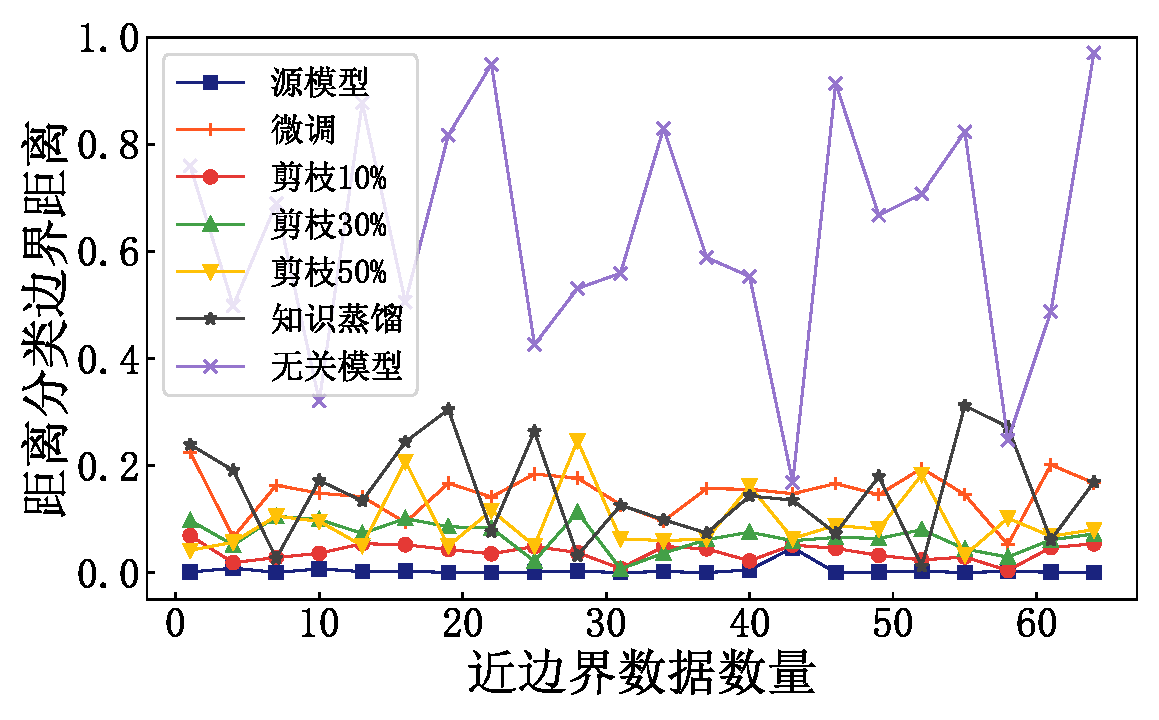
\includegraphics[width=0.49\linewidth]{CIFAR-10-4-2-distance.pdf}} 
	\subfigure{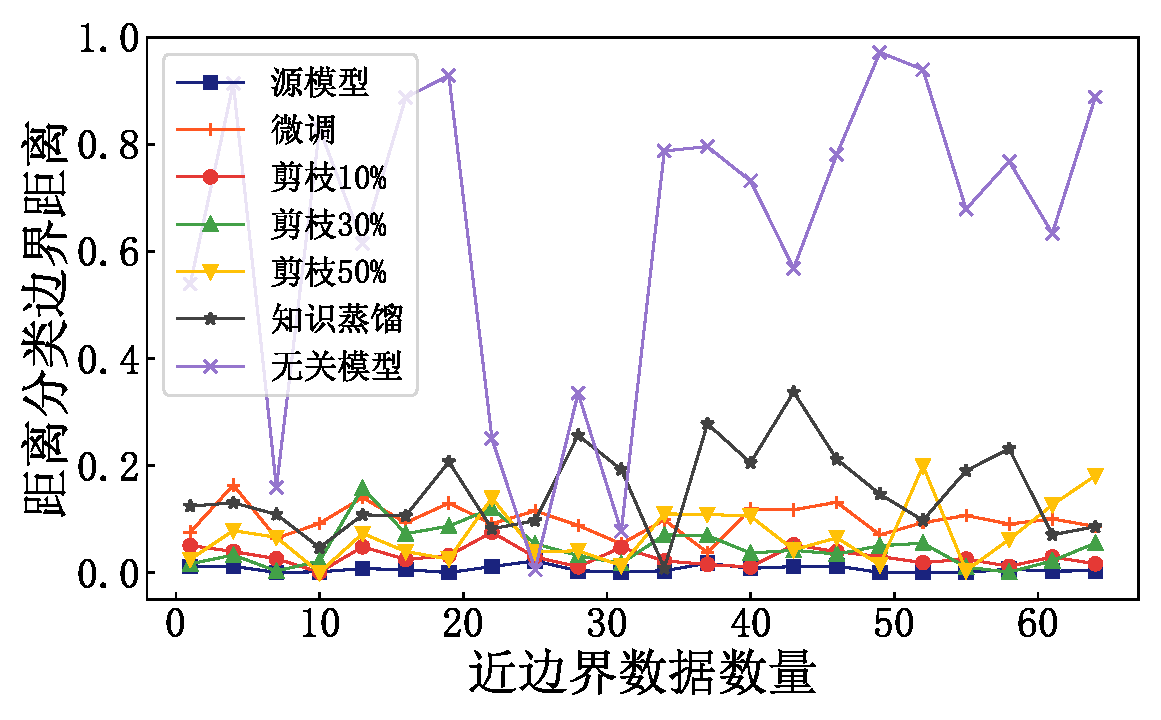
\includegraphics[width=0.49\linewidth]{CIFAR-10-4-3-distance.pdf}}
    \subfigure{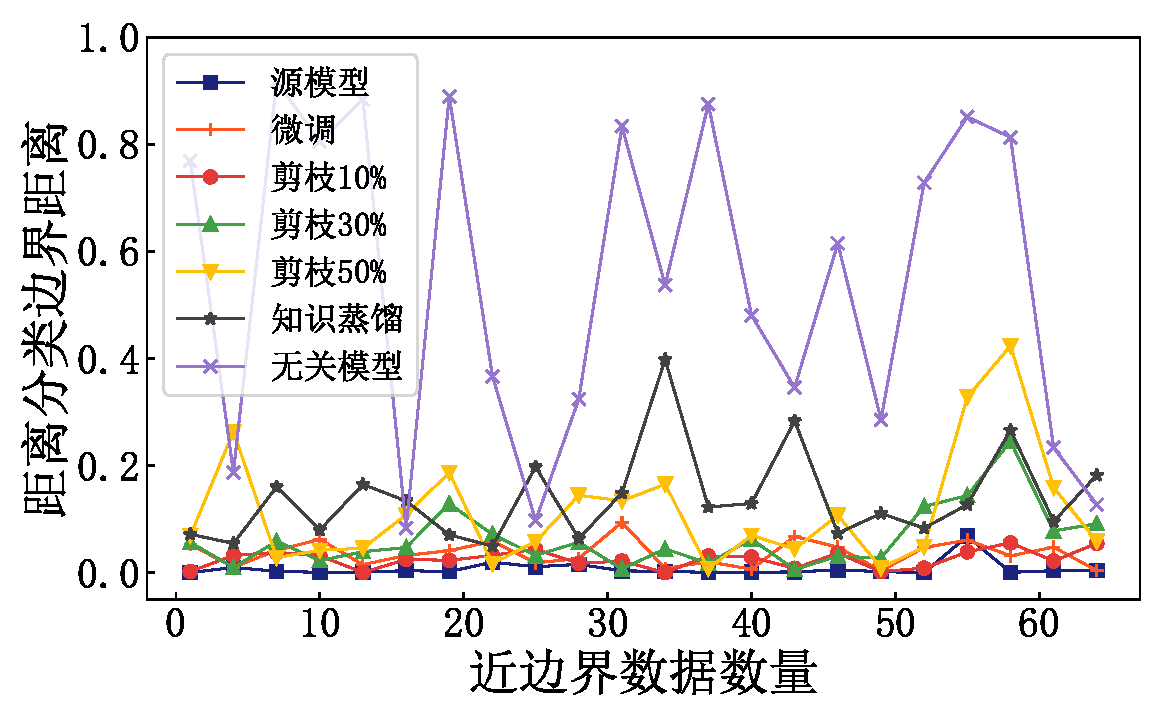
\includegraphics[width=0.49\linewidth]{CIFAR-10-4-7-distance.pdf}}
    \subfigure{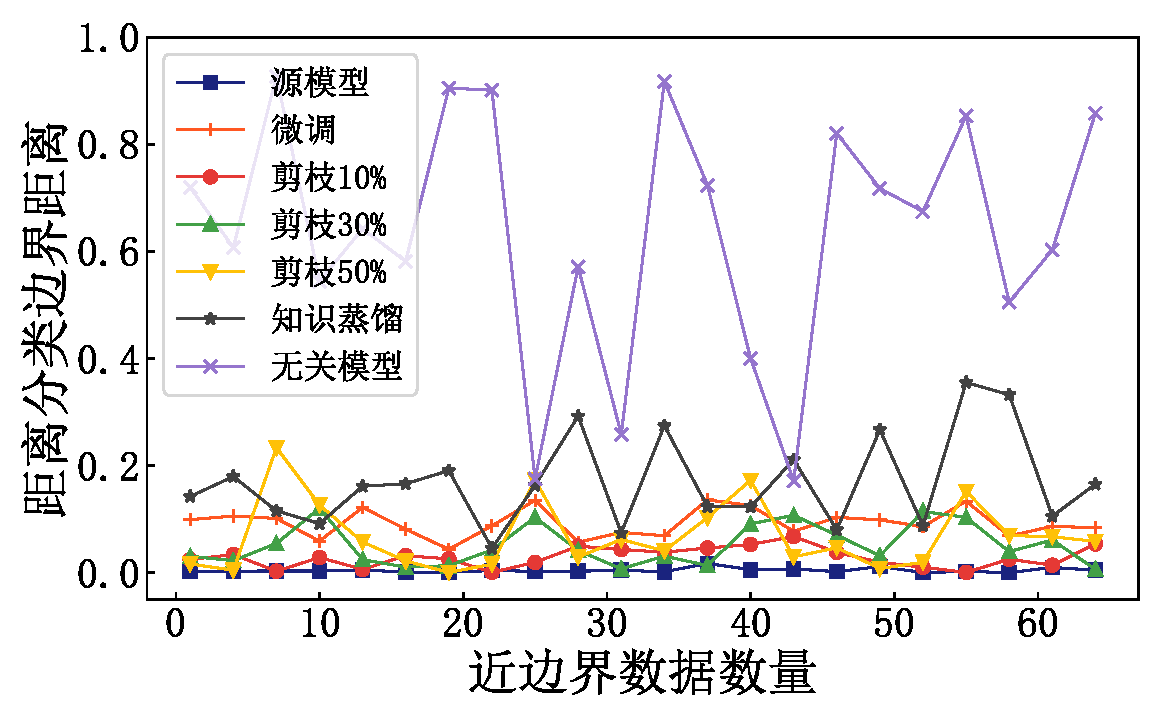
\includegraphics[width=0.49\linewidth]{CIFAR-10-5-6-distance.pdf}}
	\caption{CIFAR-10上4条不同分类边界下的近边界数据表现}
	\label{CIFAR-10上不同分类边界下的近边界数据表现}
\end{figure}

\begin{figure}[!htb]
	\centering
%	\setlength{\abovecaptionskip}{0mm}
%		\vspace{-3mm}
%	\setlength{\belowcaptionskip}{-4mm} %调整图片标题与下文距离
	\subfigure{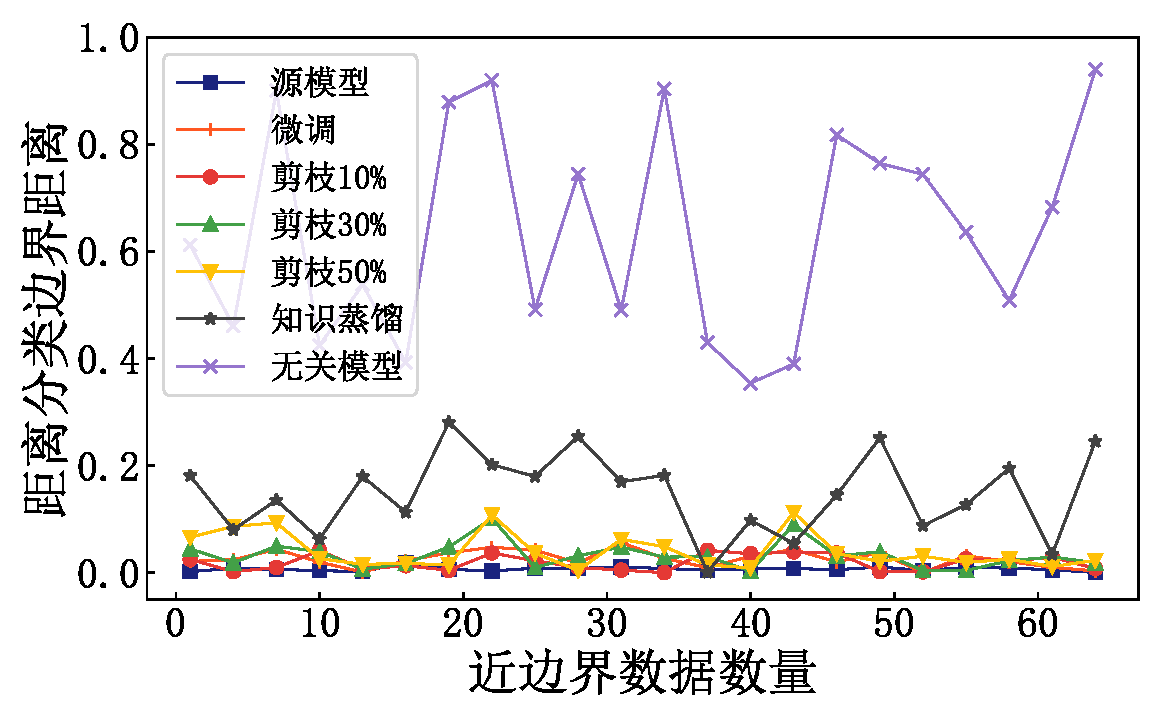
\includegraphics[width=0.49\linewidth]{Heritage-3-0-distance.pdf}} 
	\subfigure{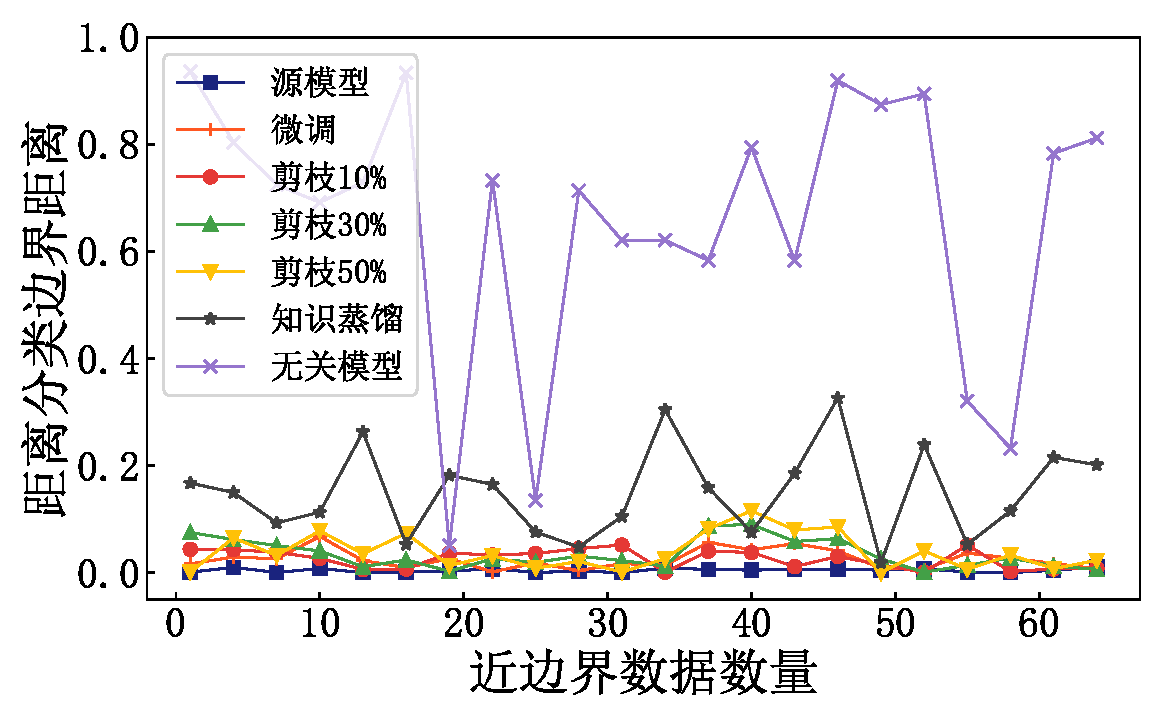
\includegraphics[width=0.49\linewidth]{Heritage-3-1-distance.pdf}} 
	\subfigure{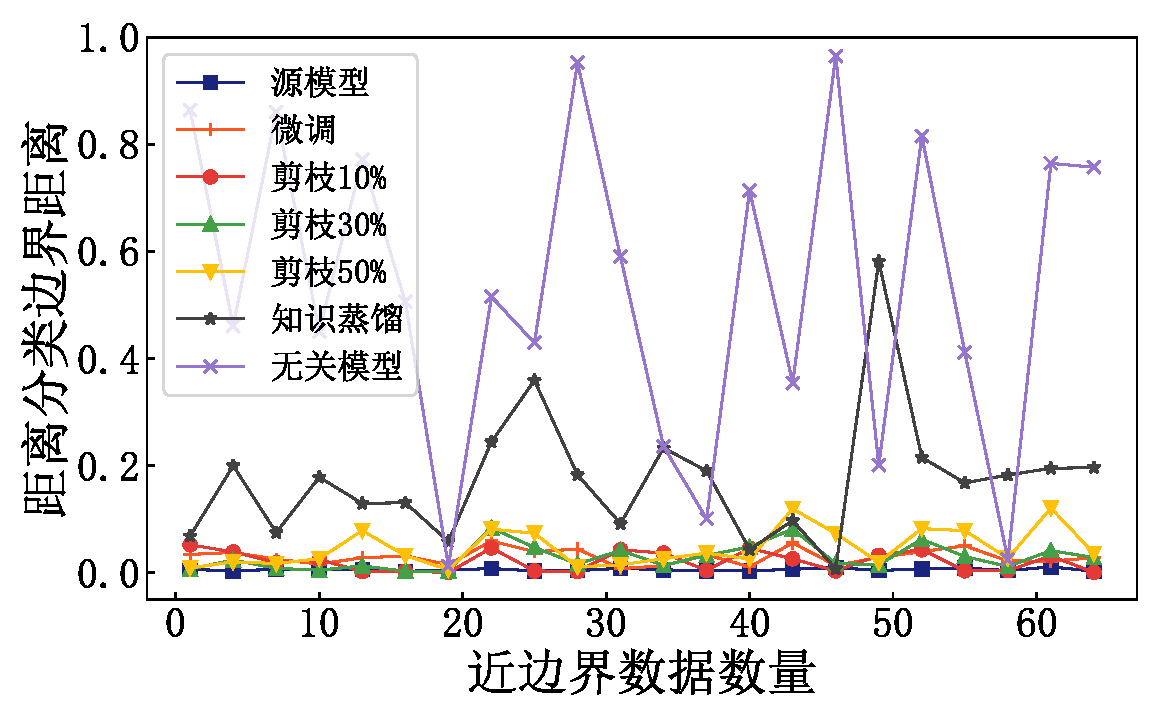
\includegraphics[width=0.49\linewidth]{Heritage-3-4-distance.pdf}} 
	\subfigure{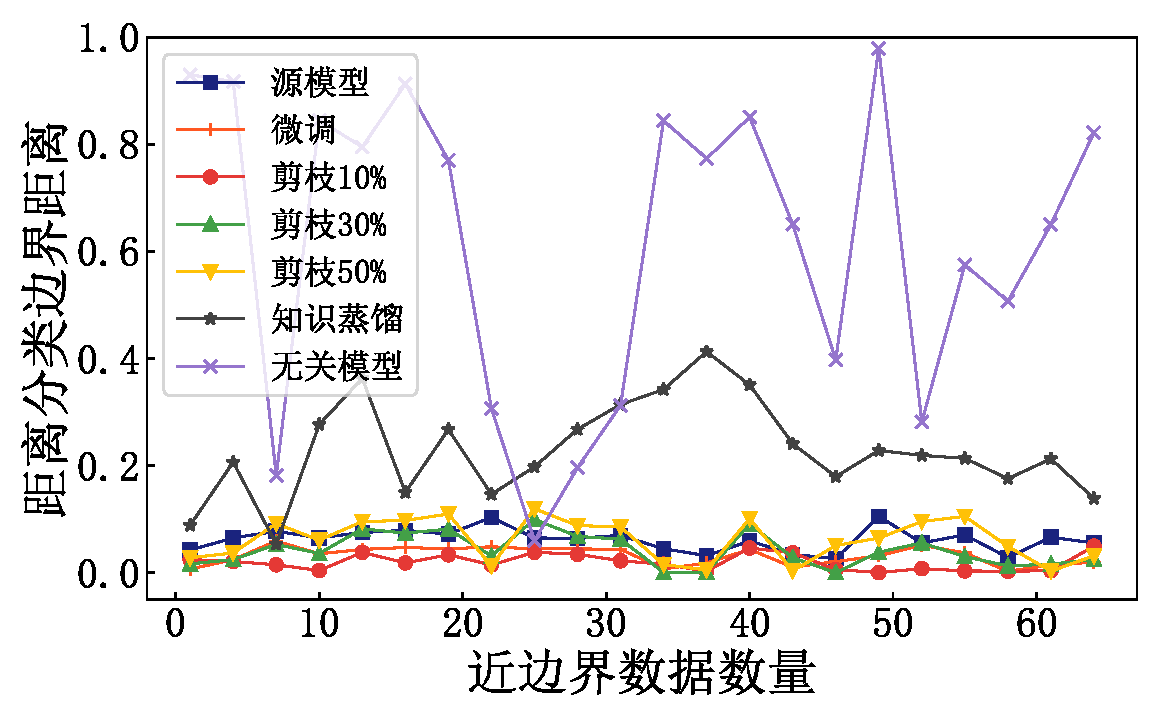
\includegraphics[width=0.49\linewidth]{Heritage-7-6-distance.pdf}} 
	\caption{Heritage上4条不同分类边界下的近边界数据表现}
	\label{Heritage上不同分类边界下的近边界数据表现}
\end{figure}

\begin{figure}[!htb]
	\centering
	\subfigure{\includegraphics[width=0.49\linewidth]{Intel\_image-3-1-distance.pdf}} 
	\subfigure{\includegraphics[width=0.49\linewidth]{Intel\_image-3-4-distance.pdf}} 
	\subfigure{\includegraphics[width=0.49\linewidth]{Intel\_image-3-5-distance.pdf}} 
	\subfigure{\includegraphics[width=0.49\linewidth]{Intel\_image-5-0-distance.pdf}}
	\caption{Intel\_image上4条不同分类边界下的近边界数据表现}
	\label{Intel-image上不同分类边界下的近边界数据表现}
\end{figure}

如图\ref{CIFAR-10上不同分类边界下的近边界数据表现},图\ref{Heritage上不同分类边界下的近边界数据表现},图\ref{Intel-image上不同分类边界下的近边界数据表现}所示, 本文提出的近边界数据在所有盗窃模型中都表现出了靠近分类边界的特点。从图中可以发现,相比于其他模型,近边界数据在源模型上距离分类边界的距离最近,这主要是三方面的原因:

1)初始的近边界样本是使用公开数据集在源模型的基础上生成的。本文从众多生成对抗性样本的方法中挑选了效果最好的CW-$L_2$方法,然后在该方法的基础上引入距离参数,改进算法的迭代过程,使之生成非常靠近目标分类边界的近边界数据。

2)使用DCGAN生成器提取近边界数据的特征后,生成了新的私有化近边界数据。在此基础上,本文设计了新的损失函数微调源模型分类边界,这使得私有近边界数据同样非常接近模型分类边界。

3)盗窃模型在从源模型派生的过程中,涉及到模型的修改。虽然这些修改操作不会使近边界数据在这些模型上失去近边界性,但是会使模型分类边界发生轻微偏移,从而近边界数据在盗窃模型上距离分类边界距离增大。


近边界数据在所有被盗模型中表现出近边界性说明近边界数据可以被继承,这跟本文使用的模型是DNN分类器有关。分类边界是分类器的重要特征,本文的近边界数据是根据分类边界构造的。即使模型窃取攻击对模型有一定程度的修改,分类器的分类边界不会发生很大的变化。因此,近边界数据拥有可继承性,在盗窃模型上同样表现出靠近分类边界的特点。这是本文提出方法的基础,因为本文方法的原理是,利用所有者的私有近边界数据和可疑对手提供的近边界数据到分类边界距离的大小来推断模型所有权(距离小者推断获得所有权)。如果私有近边界数据不表现出近边界性,那么就不适用于推断模型所有权。

从图中可以发现,相比于其他模型盗窃方法,近边界数据在知识蒸馏派生出的模型上距离分类边界距离较远。这是因为知识蒸馏对模型的修改特别大,通常来说会更换模型的架构,然后在通过蒸馏的方法进行训练。模型知识蒸馏对于其他模型知识产权保护方法也是一种挑战,但是本文提出的近边界数据在蒸馏产生的模型上仍然表现出近边界性,因此本文提出的方法对这种强修改的模型盗窃方法仍然适用。

图中还有一个点是近边界数据在无关模型上并不表现出近边界性,这是合理的。即使训练数据相同,分类边界不可能完全一样。本文提出的方法不应该对正常的无关模型产生误判,错误推断所有权。


\section{源模型微调的影响评估}\label{5.5}

本小节将对\ref{4}\ref{4.2}中使用私有近边界数据微调源模型产生的影响进行评估。本文针对不同数据集训练得到的源模型,使用不同规模的近边界数据以及不同的目标分类边界对源模型进行微调。评估指标为模型的准确率,准确率变化愈小,说明产生的不良影响越小。

\begin{table}[h]
	\centering
	%	\setlength{\arrayrulewidth}{0.5mm}
	\renewcommand\arraystretch{1.2}
	\caption{微调分类边界对准确率的影响}
	\label{table:3}
%	\resizebox{\linewidth}{!}{
%		\zihaowu
	\small
	\begin{tabular*}{14cm}{@{\extracolsep{\fill}} l c c c c}
		\toprule[1pt]
		\multirow{3}{5em}{分类边界}&\multirow{3}{5em}{数据规模} & CIFAR-10&Heritage&Intel\_image \\ 
		& & 准确率(0.886)&准确率(0.879)&准确率(0.854) \\
		\cline{3-5}	
		& &准确率&准确率&准确率 \\
		\hline
		\multirow{4}{5em}{分类边界1}&64&0.873&0.862&0.825 \\
		&128&0.862&0.858&0.829 \\
		&256&0.862&0.854&0.826 \\
		&512&0.857&0.852&0.839 \\
		\hline
		\multirow{4}{5em}{分类边界2}&64&0.871&0.867&0.843 \\
		&128&0.870&0.862&0.839 \\
		&256&0.860&0.859&0.828 \\
		&512&0.859&0.851&\textbf{0.824} \\
		\hline
		\multirow{4}{5em}{分类边界3}&64&0.871&0.865&0.841 \\
		&128&0.868&0.857&0.833 \\
		&256&0.858&0.855&0.831 \\
		&512&\textbf{0.856}&0.851&0.825 \\
		\hline
		\multirow{4}{5em}{分类边界4}&64&0.873&0.863&0.847 \\
		&128&0.873&0.860&0.843 \\
		&256&0.866&0.854&0.838 \\
		&512&0.862&\textbf{0.850}&0.831 \\
		\hline
		\multirow{4}{5em}{分类边界5}&64&0.876&0.866&0.846 \\
		&128&0.866&0.861&0.834 \\
		&256&0.868&0.857&0.829 \\
		&512&0.861&0.853&0.825 \\
		\bottomrule[1pt]
\end{tabular*}
%}
\end{table}

	
经过不同规模近边界数据微调后,源模型的准确率如表\ref{table:3}所示,每个数据集下影响最大,即准确率最低的,已在表中加粗。

从表中可以发现,几乎全部情况下,源模型微调前后的精度差没有超过3\%,这是本文方法可以接受的范围。不考虑偶然因素的影响,在大部分情况下,随着微调模型近边界数量的增多,模型准确率逐渐下降。这是合理的,因为近边界数据本身和正常训练数据不同,使用越多的异常数据参与训练,对模型的性能影响越大。但是在另一个角度,微调源模型的目的是使得私有近边界数据更加靠近目标分类边界,来提高后续推断模型所有权的置信度,所以,使用更多的近边界数据微调源模型,后续推断的效果会更好。因此,在实际情况中,微调数据规模的选择是一个模型精度和推断置信度的折衷。

表中整体情况下,模型的准确率下降不多。一方面,这是因为微调的数据和源模型的训练数据相比只是一小部分,不会对模型产生太大的影响。另一方面,在微调源模型时,本文将学习率设置较低,仅为0.0001。并且使用原始数据对模型进行交替训练,训练轮次不超过10次。所以对源模型微调之后,模型准确率没有受到很大的影响。

实验结果证明,本文的私有近边界数据在解决模型所有权保护问题时,模型具有较好的保真度。因此,使用近边界数据推断模型所有权不用担心源模型受到较大的影响,模型准确率变化在3\%以内。	
	

\section{模型所有权推断有效性评估}\label{5.6}

本文提出的方法目标是推断模型的所有权,本节将对此方法的有效性进行评估。根据本文方法的流程,模型所有者和可疑对手(可能是模型盗窃者)均需向官方仲裁机构提供各自的近边界数据,然后通过数据和模型计算到分类边界的距离,再根据\ref{4}\ref{4.3}中提到的假设检验进行进行结果对比,判断可疑模型是否从源模型派生。

在本节中,通过讨论本文方法生成的私有近边界数据与其他近边界数据在盗窃模型上的性能对比来说明本文方法的有效性。首先,本文模拟了盗窃者可能会提供的近边界数据,该数据由两部分组成,包括(1)从原始数据中挑选出的近边界数据,(2)由FGSM和CW生成的一些对抗性样本。然后针对不同的目标分类边界,进行假设检验并计算在不同数据集和不同盗窃模型上的$\Delta\mu$和$p$值,来反映成功推断所有权的置信度。本节的评估指标为$\Delta\mu$和$p$值,$\Delta\mu$愈大和$p$值愈小,推断的置信度愈高。

\begin{table}[h]
	\centering
%	\setlength{\arrayrulewidth}{0.5mm}
	\renewcommand\arraystretch{1.5}
	\caption{推断模型所有权}
	\label{table:2}
	\resizebox{\linewidth}{!}{
	\begin{tabular}{l l c c c c c c c c c c}
		
		\toprule[1pt]
\multirow{2}{5em}{数据集}&\multirow{2}{4em}{攻击方法}&\multicolumn{2}{c}{分类边界1}&\multicolumn{2}{c}{分类边界2}&\multicolumn{2}{c}{分类边界3}&\multicolumn{2}{c}{分类边界4}&\multicolumn{2}{c}{分类边界5}\\ \cline{3-12}
		                         & &$\Delta\mu$&$p$值&$\Delta\mu$&$p$值&$\Delta\mu$&$p$值&$\Delta\mu$&$p$值&$\Delta\mu$&$p$值 \\
		\hline
\multirow{6}{5em}{CIFAR-10}     &源模型    & 0.913 & $10^{-6}$ & 0.954 & $10^{-6}$ & 0.927 & $10^{-5}$ & 0.967 & $10^{-5}$ & 0.958 & $10^{-5}$   \\
								&模型微调  & 0.718 & $10^{-5}$ & 0.745 & $10^{-6}$ & 0.698 & $10^{-5}$ & 0.692 & $10^{-4}$ & 0.729 & $10^{-5}$   \\
								& 剪枝10\% & 0.572 & $10^{-5}$ & 0.487 & $10^{-5}$ & 0.458 & $10^{-5}$ & 0.533 & $10^{-4}$ & 0.512 & $10^{-4}$   \\
								&剪枝30\%  & 0.537 & $10^{-4}$ & 0.497 & $10^{-4}$ & 0.401 & $10^{-3}$ & 0.428 & $10^{-4}$ & 0.587 & $10^{-4}$   \\
								&剪枝50\%  & 0.545 & $10^{-4}$ & 0.614 & $10^{-4}$ & 0.506 & $10^{-3}$ & 0.570 & $10^{-4}$ & 0.484 & $10^{-3}$   \\
								&知识蒸馏  & 0.372 & $10^{-3}$ & 0.297 & $10^{-3}$ & 0.288 & $10^{-3}$ & 0.308 & $\pmb{10^{-2}}$ & 0.340 & $10^{-3}$   \\
		\hline
\multirow{6}{5em}{Heritage}     &源模型    & 0.876 & $10^{-5}$ & 0.845 & $10^{-5}$ & 0.859 & $10^{-4}$ & 0.801 & $10^{-4}$ & 0.837 & $10^{-5}$   \\
								&模型微调  & 0.815 & $10^{-5}$ & 0.792 & $10^{-4}$ & 0.824 & $10^{-4}$ & 0.833 & $10^{-4}$ & 0.784 & $10^{-4}$   \\
								&剪枝10\%  & 0.530 & $10^{-4}$ & 0.535 & $10^{-3}$ & 0.508 & $10^{-4}$ & 0.486 & $10^{-3}$ & 0.471 & $10^{-3}$   \\
								&剪枝30\%  & 0.491 & $10^{-3}$ & 0.452 & $10^{-3}$ & 0.469 & $10^{-4}$ & 0.470 & $10^{-3}$ & 0.427 & $10^{-4}$   \\
								&剪枝50\%  & 0.502 & $10^{-3}$ & 0.517 & $10^{-3}$ & 0.434 & $10^{-3}$ & 0.451 & $10^{-3}$ & 0.490 & $10^{-3}$   \\
								&知识蒸馏  & 0.329 & $10^{-3}$ & 0.365 & $\pmb{10^{-2}}$ & 0.238 & $10^{-3}$ & 0.310 & $10^{-3}$ & 0.274 & $10^{-3}$   \\
		\hline
\multirow{6}{5em}{Intel\_image} &源模型    & 0.859 & $10^{-5}$ & 0.896 & $10^{-4}$ & 0.872 & $10^{-4}$ & 0.899 & $10^{-4}$ & 0.914 & $10^{-4}$   \\
								&模型微调  & 0.717 & $10^{-5}$ & 0.784 & $10^{-4}$ & 0.752 & $10^{-4}$ & 0.791 & $10^{-3}$ & 0.709 & $10^{-4}$   \\
								&剪枝10\%  & 0.451 & $10^{-4}$ & 0.522 & $10^{-4}$ & 0.539 & $10^{-3}$ & 0.472 & $10^{-3}$ & 0.438 & $10^{-4}$   \\
								&剪枝30\%  & 0.407 & $10^{-4}$ & 0.415 & $10^{-4}$ & 0.346 & $10^{-3}$ & 0.382 & $10^{-3}$ & 0.395 & $10^{-3}$   \\
								&剪枝50\%  & 0.370 & $10^{-3}$ & 0.395 & $10^{-3}$ & 0.327 & $10^{-3}$ & 0.360 & $10^{-3}$ & 0.458 & $10^{-3}$   \\
								&知识蒸馏  & 0.336 & $\pmb{10^{-2}}$ & 0.395 & $10^{-3}$ & 0.360 & $\pmb{10^{-2}}$ & 0.308 & $10^{-3}$ & 0.287 & $\pmb{10^{-2}}$   \\
		\bottomrule[1pt]		
	\end{tabular}
}
\end{table}

不同数据集下,针对不同分类边界,所有者的私有近边界数据和其他近边界数据计算得到的$\Delta\mu$和$p$值如表\ref{table:2}所示,不同目标分类边界下$p$值的最小情况已在表格中加粗。

从表中可以发现,在每个数据集,每条分类边界上$p$值呈从上到下增大的趋势,$\Delta\mu$呈减小趋势。尽管如此,在全部情况中,$p$值均低于0.05,即至少有95\%以上的置信度,推断盗窃模型从源模型派生。即本文的方法在不同的模型窃取方法中推断模型的所有权,均有显著的效果,至少有95\%以上的置信度确定可疑模型是盗窃模型。

在假设检验中,$p$值越小,$\Delta\mu$越大说明结果越可靠,推断的置信度越高。表中从上到小$p$值减小是因为这些模型窃取方法对模型的修改逐渐增大,尤其是知识蒸馏。模型知识蒸馏是本文方法的最大挑战,也同样是其他研究面临的巨大挑战。从表中,可以观察到本文提出的的方法始终可以将蒸馏模型推断为被盗模型。因此,实验结果表明使用私有的近边界数据来推断模型所有权的方法对大多数模型盗窃技术都是可靠的,模型被盗窃的置信度至少达到95\%,证明了本文方法的有效性和鲁棒性。


\section{近边界数据规模可伸缩性评估}\label{5.7}

本节将测试使用不同规模的近边界数据,在推断模型所有权时的可伸缩性。本文提出的方法需要对数据进行采样从而进行假设检验,通常情况下,样本数量越大,检验过程中因随机因素而产生的不利影响就会越小,更能准确的推断可疑模型所有权。

\begin{figure}[!htb]
	\centering
	\subfigure{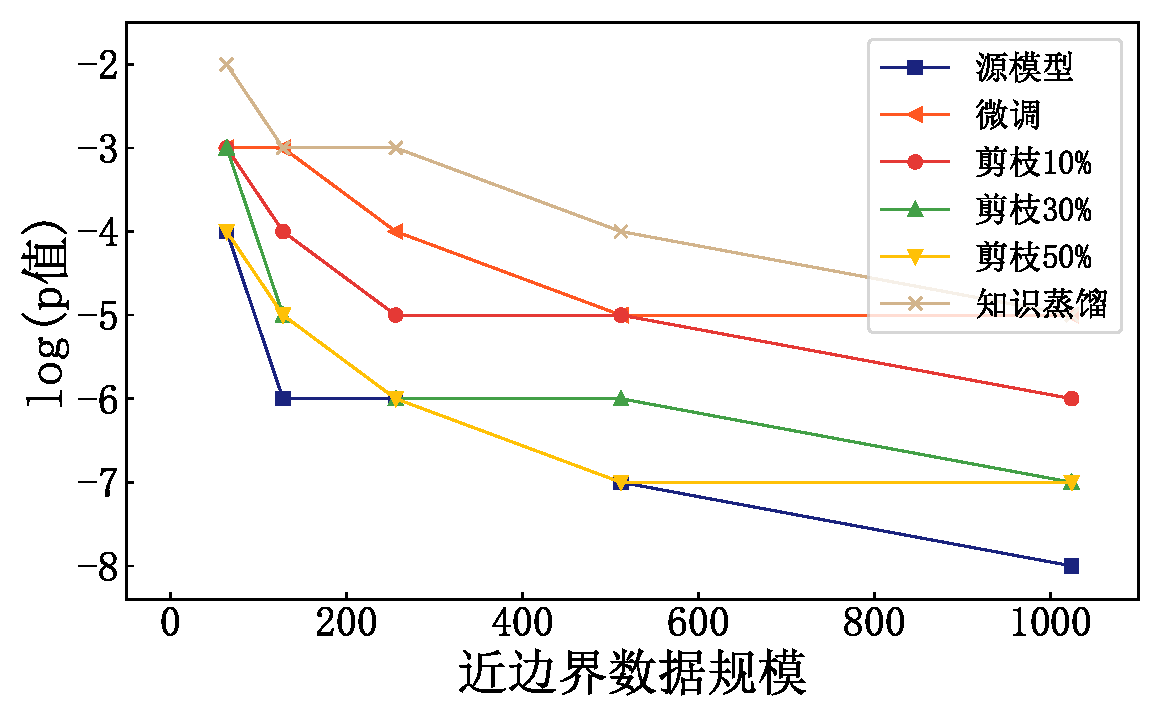
\includegraphics[width=0.49\linewidth]{CIFAR-10-4-2-p-value.pdf}} 
	\subfigure{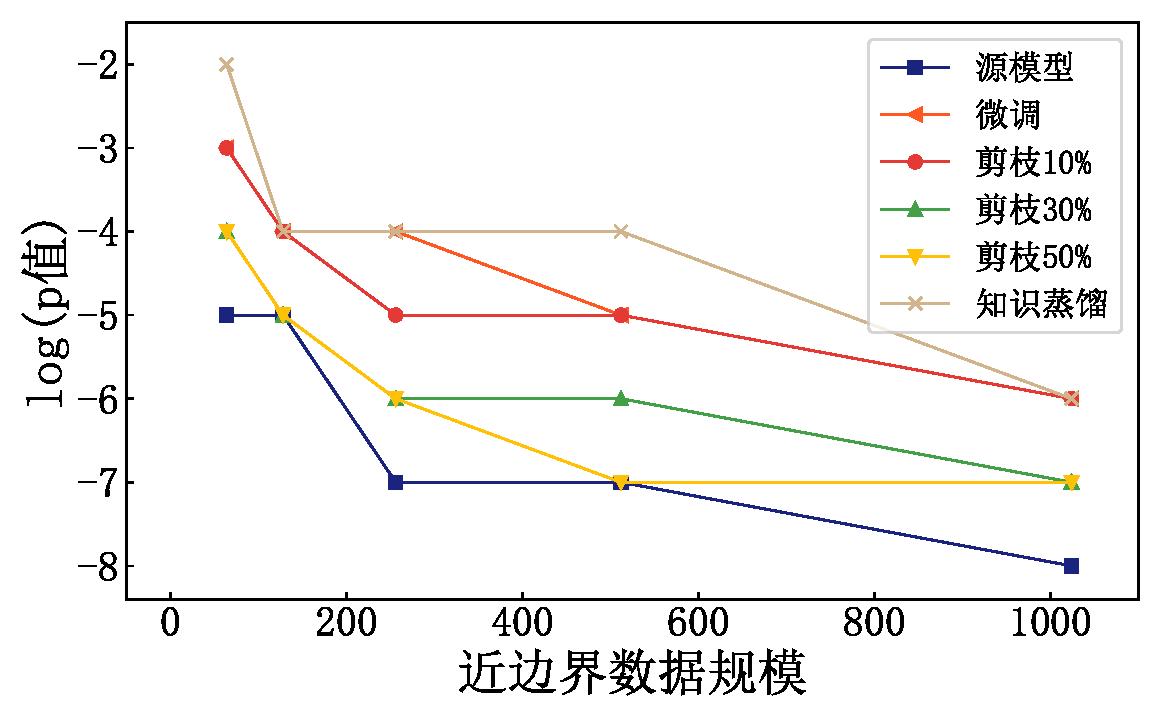
\includegraphics[width=0.49\linewidth]{CIFAR-10-4-3-p-value.pdf}}
	\subfigure{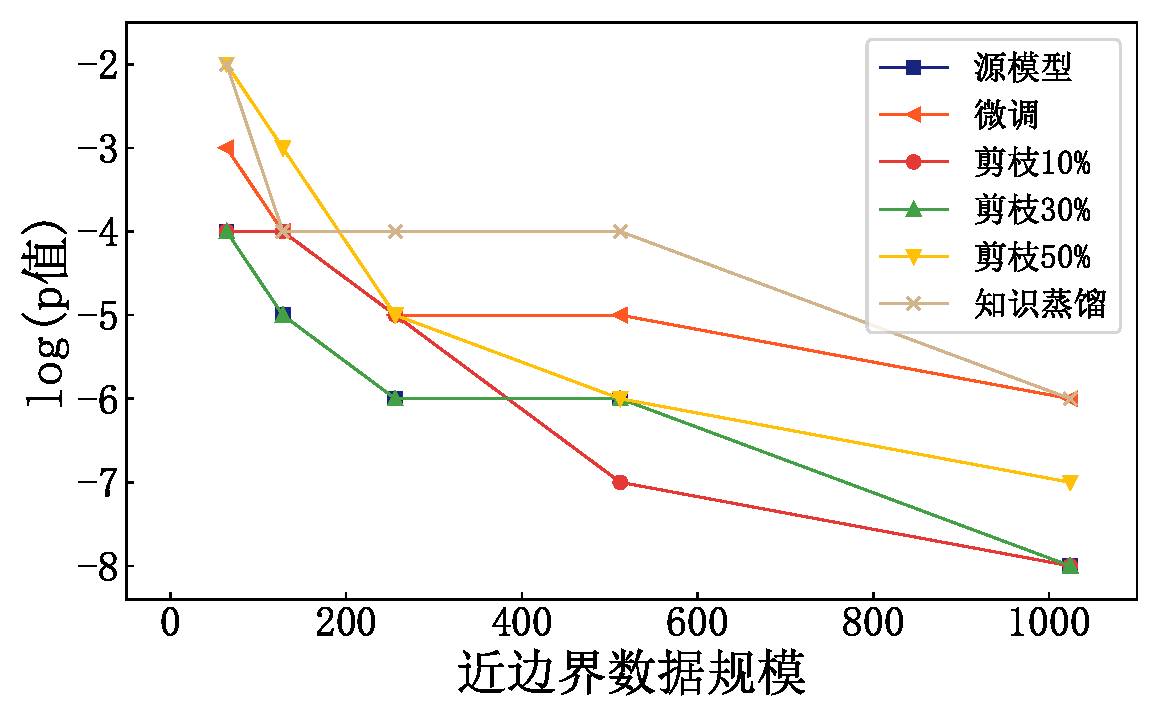
\includegraphics[width=0.49\linewidth]{CIFAR-10-4-7-p-value.pdf}}
	\subfigure{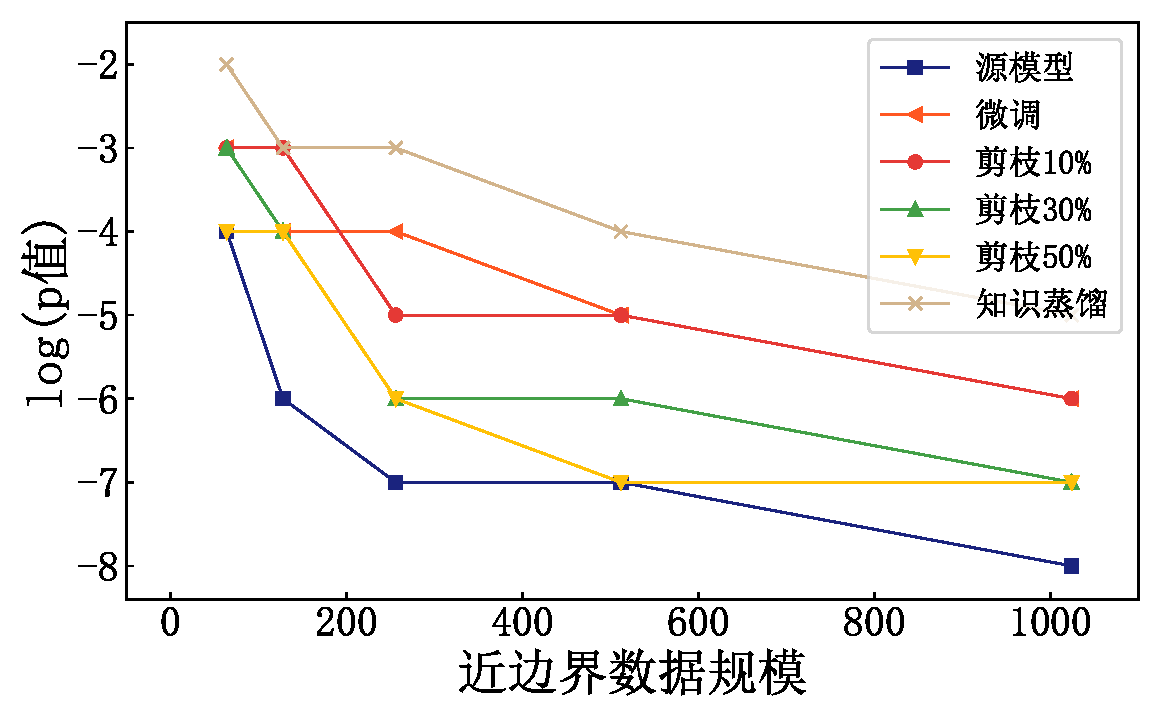
\includegraphics[width=0.49\linewidth]{CIFAR-10-5-6-p-value.pdf}} 
	\caption{CIFAR-10上4条不同分类边界下的近边界数据规模可伸缩性}
	\label{CIFAR-10上推断模型所有权的扩展性}
%	\setlength{\abovecaptionskip}{7mm}
\end{figure}

\begin{figure}[!htb]
	\centering
	\subfigure{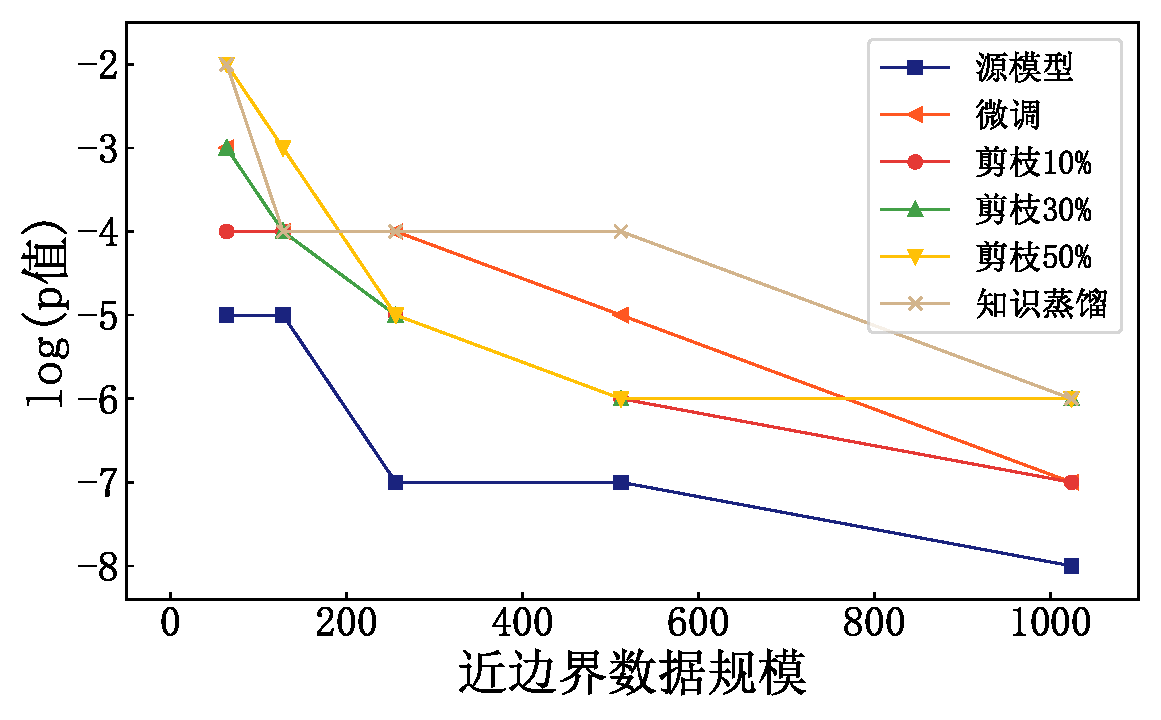
\includegraphics[width=0.49\linewidth]{Heritage-3-0-p-value.pdf}} 
	\subfigure{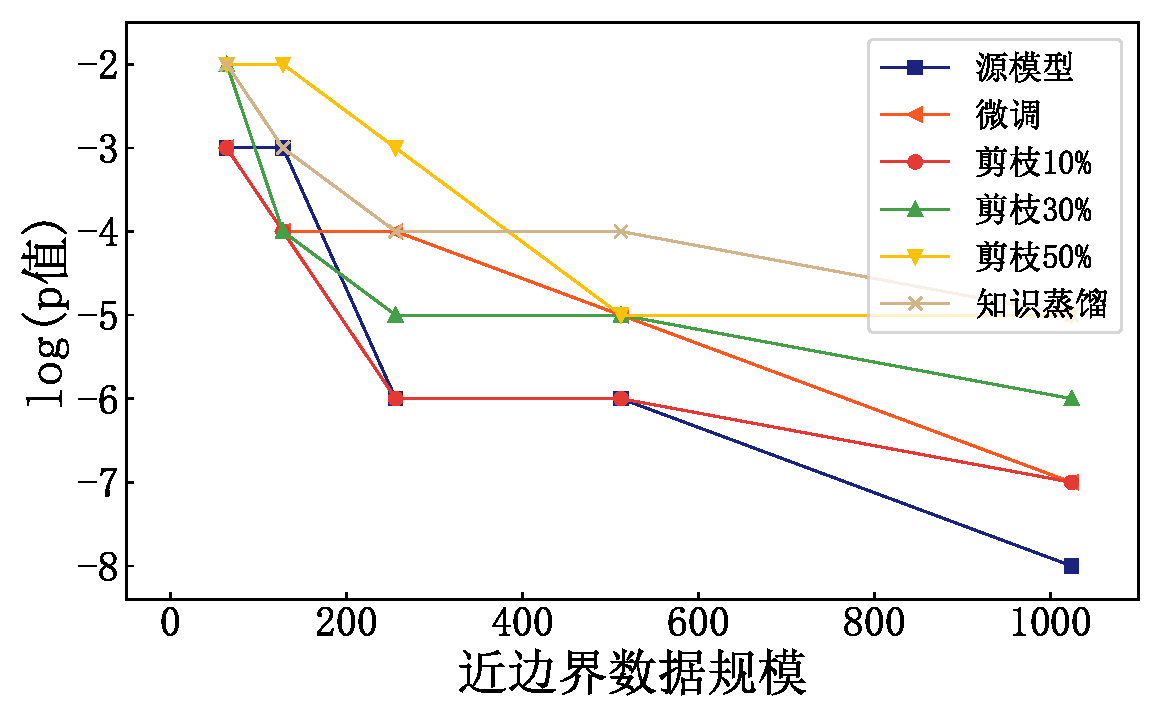
\includegraphics[width=0.49\linewidth]{Heritage-3-1-p-value.pdf}} 
	\subfigure{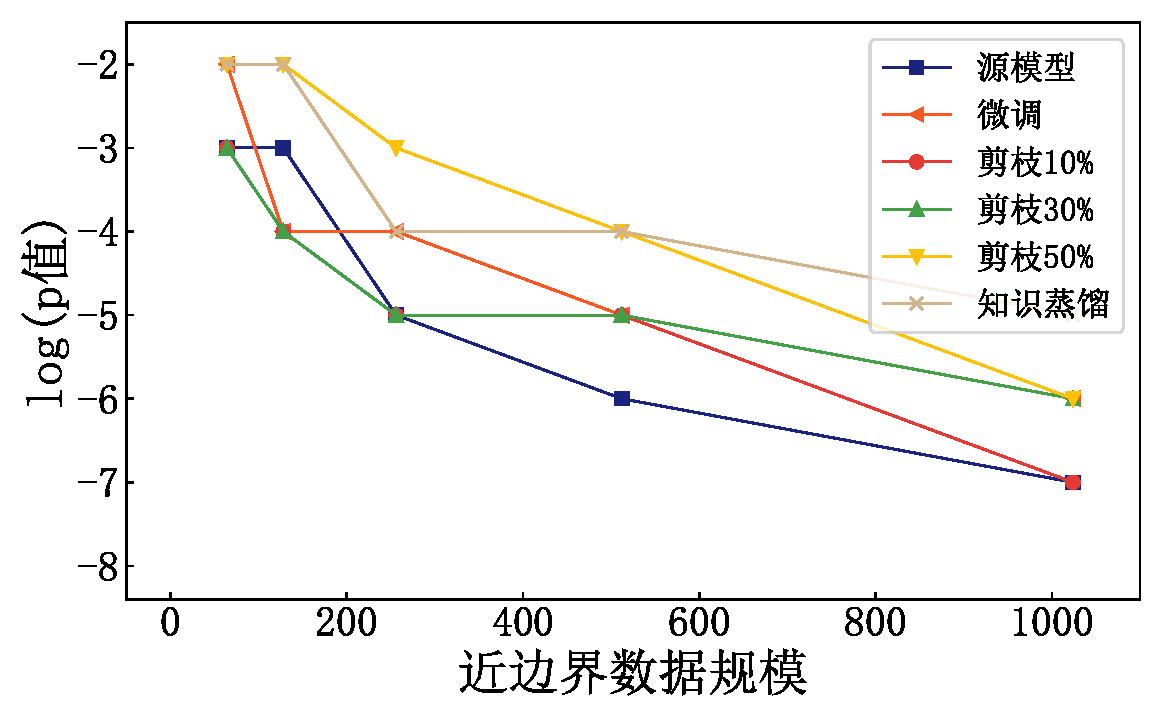
\includegraphics[width=0.49\linewidth]{Heritage-3-4-p-value.pdf}} 
	\subfigure{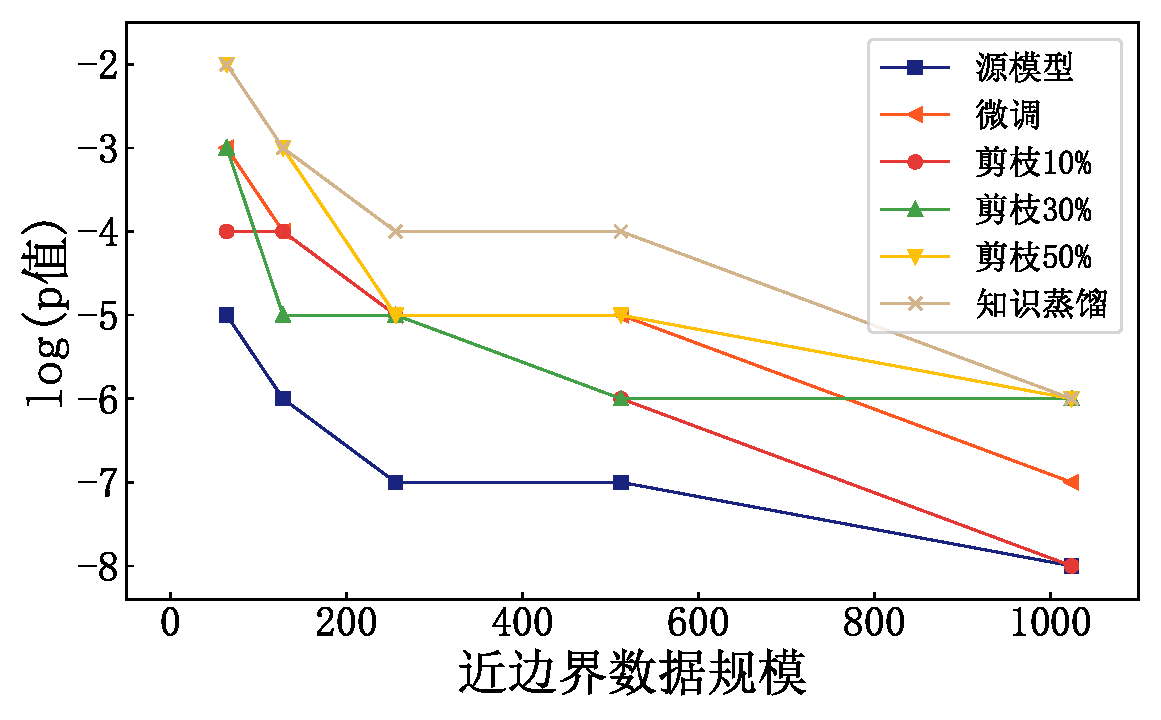
\includegraphics[width=0.49\linewidth]{Heritage-7-6-p-value.pdf}} 
	\caption{Heritage上4条不同分类边界下的近边界数据规模可伸缩性}
	\label{Heritage上推断模型所有权的扩展性}
%	\setlength{\abovecaptionskip}{7mm}
\end{figure}

\begin{figure}[!htb]
	\centering
	\subfigure{\includegraphics[width=0.49\linewidth]{Intel\_image-3-1-p-value.pdf}} 
	\subfigure{\includegraphics[width=0.49\linewidth]{Intel\_image-3-4-p-value.pdf}} 
	\subfigure{\includegraphics[width=0.49\linewidth]{Intel\_image-3-5-p-value.pdf}} 
	\subfigure{\includegraphics[width=0.49\linewidth]{Intel\_image-5-0-p-value.pdf}} 
	\caption{Intel\_image上4条不同分类边界下的近边界数据规模可伸缩性}
	\label{Intel-image上推断模型所有权的扩展性}
%	\setlength{\abovecaptionskip}{7mm}
\end{figure}

如图\ref{CIFAR-10上推断模型所有权的扩展性},图\ref{Heritage上推断模型所有权的扩展性},图\ref{Intel-image上推断模型所有权的扩展性}所示,$p$值在不同数据集,不同分类边界上,随着近边界数据规模的增大而减小,而$p$值越小说明假设检验能够以更高的置信度确定可疑模型是被盗模型。

本文的方法在进行假设检验前,需要将私有的近边界数据和可疑对手的近边界数据分别通过可疑模型,计算到目标分类边界的距离。可疑对手的近边界数据是通过从原始数据挑选和FGSM,CW生成的对抗性样本组成的。因此,由于随机因素的影响,存在一小部分可疑对手提供的数据到分类边界的距离和所有者提供的私有近边界数据相近,甚至更小的情况,这会对本文的方法产生一定的干扰。随着测试样本规模的增大,这种随机因素的影响会被逐渐消除。从图中可以发现,随着近边界数据规模的增大,$p$值逐渐减小。但这并不说明本文的方法对小规模数量的近边界数据缺少鲁棒性,从图中可以发现,即使在数据量为64的情况下,$p$值仍然小于0.05,这证明本文的方法对于小数样本量同样有显著的效果,可以高置信度的推断模型所有权。\\

\textbf{方法设计目标分析}

以下对\ref{4}\ref{4.3}中提出的方法设计目标是否达到进行分析。

1)\textbf{精确性:}本文方法对模型精确性的影响主要来源于使用近边界数据微调源模型目标分类边界,这是为了增加推断模型所有权的置信度。\ref{5.5}评估了不同规模近边界数据微调源模型的影响,各种情况下,模型精度下降不超过3\%。

2)\textbf{可继承性:}\ref{5.4}中通过16组测试,验证了近边界数据的可继承性,这是选择近边界数据进行所有权推断的原因。另外,无关模型没有对近边界数据没有表现出明显特征,表明本文的方法不会产生误判。

3)\textbf{有效性:}\ref{5.6}中,使用私有近边界数据和其他近边界数据,针对各种盗窃模型,计算距离结果。然后对双方的结果进行假设检验,结果表明了本文的方法推断所有权的有效性。此外,与过去工作中利用模型水印和指纹验证模型所有权相比,本文方法使用数据在对应模型上结果作为所有权推断依据,结果的可比性和唯一性可以有效避免歧义攻击。

4)\textbf{鲁棒性:}\ref{5.4}和\ref{5.6}中,对各种盗窃模型进行了测试,本文的方法均有效,表明了本文方法的鲁棒性。

5)\textbf{不可获得性:}本文使用改进的CW-$L_2$构造了初始近边界数据,并且设计了基于DCGAN的特征提取器,私有化近边界数据。模型盗窃者由于不知道约定的分类边界,需要大量的测试,这会导致极大的成本代价。不存在无法攻击的防御方法,但可以从攻击成本上进行约束。

6)\textbf{高效性:}本文方法使用模型所有者和盗窃者提供的近边界数据输入模型后计算结果,然后通过假设检验的方式对比结果差异。该过程执行方便,不涉及复杂的处理,可以高效的进行。

\section{本章小结}

本章在CIFAR-10,Heritage,Intel\_image这三个数据集上对本文提出的方法进行了全面的测评与分析。第二节,对不同初始近边界数据生成算法进行对比,结果表明CW-$L_2$方法可以满足本文的需求,生成足够靠近目标分类边界的近边界数据。第三节,对近边界数据私有化方法进行了对比,结果表明基于DCGAN的网络架构可以更好的提取数据样本特征,生成新的靠近分类边界的数据。第四节,通过16组测试验证了近边界数据的可继承性,这是本文方法选择近边界数据作为推断数据的原因。第五节,测试了微调分类边界对模型准确率的影响,保护模型知识产权的方法不应该对模型精度造成很大的影响,否则该方法失去了意义。第六节,评估了本文方法推断模型所有权的有效性,结果表明该方法对不同的模型盗窃方法均能以95\%以上的置信度推断可疑模型是盗窃模型。第七节,对假设检验的样本规模进行了扩展,在更大规模的情况下,本文的方法会更加有效,当然,该方法也适用于类似64的小样本数据情况。
